\documentclass[11pt]{beamer}
\usetheme{Darmstadt}
\useoutertheme{split}
\useoutertheme{miniframes}
\usepackage{hyperref}
\usepackage{bm}
\usepackage{times}
\usefonttheme{structurebold}
\usepackage{array}
\usepackage[english]{babel}
\usepackage{amsmath,amssymb}
\usepackage[latin1]{inputenc}

%Code snippets and syntax highlighting
\usepackage{listings}
%Settings for Listings
\lstset{
  language=Python,
  basicstyle=\ttfamily,
  keywordstyle=\color{blue}\ttfamily,
  stringstyle=\color{red}\ttfamily,
  commentstyle=\color{green}\ttfamily,
  morecomment=[l][\color{magenta}]{\#}
}

\usepackage{array}
\usepackage{threeparttable}
\usepackage{colortbl}
\usepackage{multirow}
\usepackage{amsthm}
\usepackage{float,graphicx,color}
\newtheorem*{thm}{Theorem}
\theoremstyle{definition}
%\numberwithin{equation}{section}
\newtheorem*{defn}{Definition}
\newcommand\boldline{\arrayrulewidth{1pt}\hline}
\newcommand\ve{\varepsilon}


\setbeamercovered{dynamic}

\title[Multi-country OLG]{Multi-Country OLG model}
\author[Phillips, Clawson and Olmstead]{Kerk Phillips, Jeff Clawson and James Olmstead}
\date{October 1, 2015}


\begin{document}

\frame{\titlepage}


\section{Intro}

\frame{
\frametitle{Introduction}
  \begin{itemize}
    \item<1-> Primary research question:
      \vspace{2mm}
      \begin{itemize}

        \item  What the effects of different tax policy in various countries on the rest of the world?

      \end{itemize}
    \vspace{4mm}

    \item<2->  What we are doing:
      \vspace{2mm}
      \begin{itemize}
        \item Reconstructing OLG model of a large open economy in Python developed by various authors
      \vspace{2mm}
        \item Model economies of 7 different regions (U.S.A, E.U., Japan, China, India, Russia, and Korea) and how they interact
      \end{itemize}
    \vspace{4mm}


    \item<3-> Motivation
      \vspace{2mm}
      \begin{itemize}
        \item Inform policy makers of macroeconomic impact of various tax reforms
        \item Incorporate theory into general OSPC model
      \end{itemize}
  \end{itemize}
}

\frame{
\frametitle{Literature}
\begin{itemize}
\item<1->Auerbach and Kotlikoff (1987), "Dynamic Fiscal Policy"
\vspace{4mm}
\begin{itemize}
\item Book that developed multi-generational model to examine effects of tax policy
\end{itemize} 
\vspace{4mm}
\item<2-> Fehr, Jokisch,  and Kotlikoff (2008), "Dynamic Globalization and Its Potentially Alarming Prospects for Low-Wage Workers"
\vspace{4mm}
\begin{itemize}
\item 6-good, 5-region general equilibrium, life-cycle model that focuses on wage difference between low-skill and high-skill workers

\end{itemize} 

\end{itemize}
}

\frame{
\frametitle{Literature}
\begin{itemize}
\item<1-> Fehr, Jokisch, Kambhampati, and Kotlikoff (2013), "Simulating the Elimination of the U.S. Corporate Income Tax"
\vspace{2mm}
\begin{itemize}
\item Simulates corporate tax reform in a single good, five-region (U.S., Europe, Japan, China,
India) model, featuring skilled and unskilled labor, detailed region-specific demographics and fiscal policies

\end{itemize} 
\vspace{4mm}
\item<2-> Benzell, Goryunov, Kazakova, Lagarda, Nesterova, Kotlikoff, and Zubarev (2014), "Simulating Russia's Challenging Transition"
\vspace{4mm}
\begin{itemize}
\item Simulated Russia's economy with focus on fossil fuels that included U.S., China, India, E.U., and Japan+
\end{itemize} 

\end{itemize}
}


\frame{
\frametitle{Answer to research question}
  \begin{itemize}
    \item<1-> .......We don't have an answer to our research question yet since we are still building the model in Python
    \vspace{4mm}
    \item How we are building the model:
      \begin{itemize}
        \vspace{4mm}
        \item Stage 1. Simple OLG Model
        \vspace{2mm}
        \item Stage 2. Demographics and Growth
  \end{itemize}
 \end{itemize}
}


\section{Data and Parameters}

\frame{
\frametitle{The Data}
  \begin{itemize}
    \item Time t=0 is year 2008
    \vspace{1mm}
    \item Initial population of each country by age
    \vspace{1mm}
    \item Net migration by age
    \vspace{1mm}
    \item Fertility rates by age
    \vspace{1mm}
    \item Mortality rates by age
    \vspace{1mm}
    \item Data for taxes, government, etc. not yet in model
    \vspace{1mm}
    \item<2-> All the data (except for Korea) comes from Kotlikoff and coauthors and was pulled from a variety of data sources.
  \end{itemize}
}

\frame{
\frametitle{Korean Data}
  \begin{itemize}

    \item<1-> 2008 population by age:
      \begin{itemize}
        \vspace{1mm}
        \item Fix a sixth degree polymonial of weighted average of 2005 and 2010 census data
       \end{itemize}
        \vspace{1mm}

    \item<2-> Fertility rates:
      \begin{itemize}
        \vspace{1mm}
        \item 2005-2010 data grouped into 5 age brackets
        \item Fit to sixth degree polynomial for continuous function
       \end{itemize}

        \vspace{1mm}


    \item<3-> Mortality rates:
      \begin{itemize}
        \vspace{1mm}
        \item 2005-2010 mortality hazard data fit to fourth degree polynomial

       \end{itemize}
        \vspace{1mm}

    \item<4-> Immigration rates:
      \begin{itemize}
        \vspace{1mm}
        \item Used 2012 net migration data by age
       \end{itemize}
        \vspace{1mm}

    \item<5-> Government data:
      \begin{itemize}
        \vspace{1mm}
        \item Taken from various government websites like U.S. Social Security Administration, Global Property Guide, etc. 
       \end{itemize}

  \end{itemize}
}

\frame{
\frametitle{Parameters}
  \begin{itemize}
    \item<1-> Most parameters used in the model taken from papers by Kotlikoff and coauthors
    \vspace{4mm}
    \item<2-> $\bm{\beta}$ (Time preference ratio) and $\bm{\delta}$ (depreciation rate) are functions of S to help with convergence
    \vspace{4mm}
    \item<3-> $\bm{\xi}$ (Convex conjugate convergence parameter) adapts to more difficult problems
  \end{itemize}
}


\section{The Model}

\frame{
\frametitle{Model Beginnings}
\begin{itemize}
\vspace{4mm}
\item Began by taking Larry Kotlikoff's original Fortran Code and making a direct translation to Python.
\vspace{4mm}
\item Posed problems because of the organization and differences between indexing arrays in Python and Fortran.
\vspace{4mm}
\item Instead we decided to not do the translation and instead went with coding from the ground up in Python.

\end{itemize}
}

\frame{
\frametitle{Model Summary}
\begin{itemize}
\vspace{4mm}

\item Dynamic Life-Cycle Model
\vspace{1mm}
	\begin{itemize}
	\item 80-period lived agents
	\vspace{1mm}
	\item 7 Countries: U.S.A, E.U., Japan, China, India, Russia, Korea
	\vspace{1mm}
	\item We are building up to have similiar models as Kotlikoff papers
	\end{itemize}

\vspace{2mm}
\item<2-> What the Python code does:
\vspace{1mm}
	\begin{itemize}
	\item<2-> Demographic/population dynamics steady state prior to rest of model
	\vspace{1mm}
	\item<3-> Get equilibrium for fixed steady-state year
	\vspace{1mm}
	\item<4-> Solve for transition path using TPI
	\end{itemize}

\end{itemize}
}

\frame{
\frametitle{Demographics}
\begin{itemize}
\item The population of age s people in country i in period t is represented by $N_{ist}$
\item Births occur as fractions of people born each period. This fraction born to people of age s in country i in period t is $f_{ist}$
\begin{itemize}
\item People stop having kids at age 45 and begin at age 23.

\end{itemize}
\item Mortality rates, as stated before, are represented as $\rho_{ist}$
\begin{itemize}
\item People don't begin to die until age 68, this way, parents never outlive their children.

\end{itemize}

\item Labor is mobile, migration occurs every year up until people are age 68 and is idential every year
\vspace{3mm}
\item Bequests
\begin{itemize}
\item Those the die leave their assets and they are spread equally across all households.
\end{itemize}
\end{itemize}
}


\frame{
\frametitle{Stationarization of Demographics}
\begin{itemize}
\item Why we must stationarize the population growth:
\begin{itemize}
\vspace{1mm}
\item In order to calculate a steady state, population growth rates must be constant
\vspace{1mm}
\item Population projections are very hard beyond 50-60 years
\end{itemize}
\vspace{2mm}
\item<2-> How we do it:
\begin{itemize}
\vspace{1mm}
\item<3-> Use population shares rather than total population
\vspace{1mm}
\item<4-> Fix a transition year
\vspace{1mm}
\item<5-> After transition year, fertility, mortality, and immigration rates are same across countries
\vspace{1mm}
\item<6-> Iterate as many years as needed for population shares to converge
\end{itemize}

\end{itemize}
}

\begin{frame}
\frametitle{Initial Year Population Share Distribution}
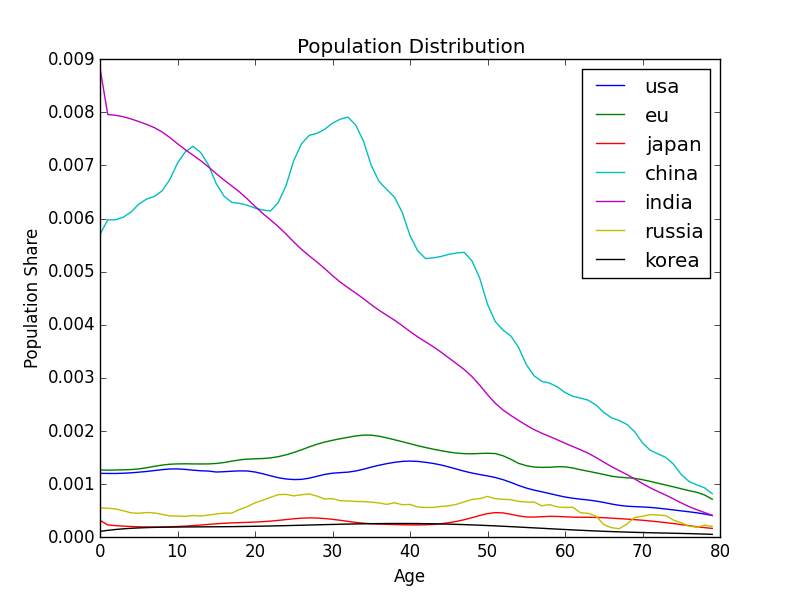
\includegraphics[scale=0.47]{popdist.png}
\end{frame}

\begin{frame}
\frametitle{Population Share Equilibrium Transition}
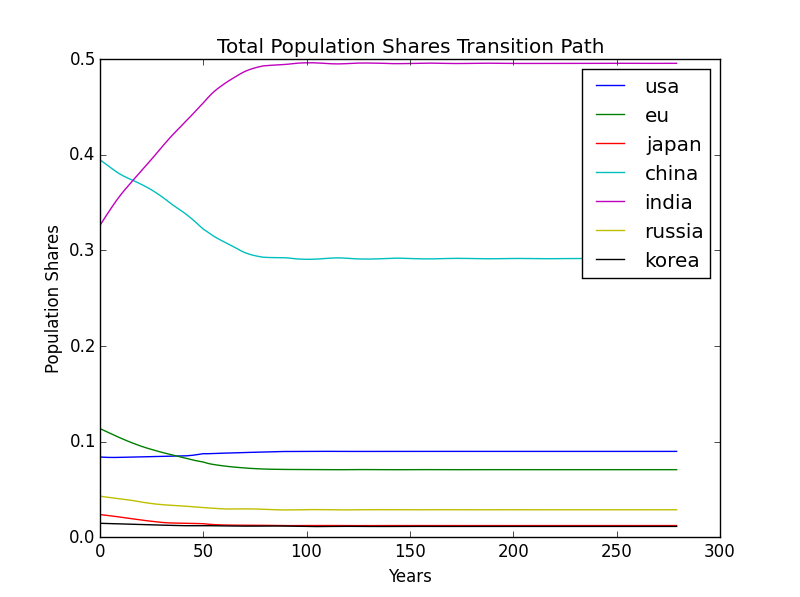
\includegraphics[scale=0.47]{popshares.png}
\end{frame}


\frame{
\frametitle{Households}
\begin{itemize}
\item Households Maximize Utility according to:
\vspace{2mm}
\begin{equation}
\max_{\{c_{i,s+j,t+j}\}_{j=0}^{S-s}} U_{ist} = \sum_{j=0}^{S-s} \beta^j \rho _{ist}^c\frac{1}{1-\sigma} c_{i,s+j,t+j}^{1-\sigma} \nonumber
\end{equation}
subject to the budget constraint in each period
\begin{equation}
\hat c_{ist} = w_{it} e_{st} + (1+r_{1t}-\delta)\hat a_{ist} + \hat{bq}_{ist} - \hat a_{i,s+1,t+1}e^{g^A} ; \forall i,s 
\end{equation}
\vspace{2mm}
\item Mortality Function:

\begin{equation}
\rho^c_{i,s+J,t+J} = \prod_{j=1}^{J}(1- \rho_{i,s+j,t+j})\nonumber
\end{equation}



\end{itemize}
}

\frame{
\frametitle{Firms}
\begin{itemize}
\item The Representative Firm Maximizes According to:
\vspace{2mm}
\begin{equation}
\max_{n_{i,t},k_{i,t}} \Pi_{ist} = k+{it}^\alpha(A_i n_{it})^{1-\alpha} -w_{it}n_{it}-r_{it}k_{it}\nonumber
\end{equation}

\end{itemize}
}

\section{Solving the Model}

\frame{
\frametitle{Trade}
\begin{itemize}
\item Mechanism of Trade:
\begin{itemize}
\item Trade occurs through capital

\item Total amount of foreign-owned domestic capital sums to zero. (In other words, our model represents the entire world)
\end{itemize}
\vspace{2mm}

\item There is one Global Interest Rate
\begin{equation} \label{Eq_requal}
r_{it} = r_t
\end{equation}


\end{itemize}
}


\frame{
\frametitle{Dynamic equations}


\begin{align}
g^N_t & = \sum_{i=1}^I \sum_{s=1}^S \hat N_{ist} (f_{ist}+m_{ist}-\rho_{ist}) ; \forall i\\
\hat N_{i,1,t+1} & = e^{-g^N_t}\sum_{s=23}^{45} \hat N_{ist} f_{ist} ; \forall i\\
\hat N_{i,s+1,t+1} & = e^{-g^N_t}\hat N_{ist} (1+m_{ist}-\rho_{ist}); \forall i, 1<s\le S \\
\hat k_{it} & = \sum_{s=1}^S \hat a_{ist} \hat N_{ist} - \hat k_{it}^f; \forall i \\
\hat n_{it} & = \sum_{s=1}^S e_{is} \hat N_{ist}; \forall i
\end{align}
}

\frame{
\frametitle{Dynamic equations 2}


\begin{align}
\hat y_{it} & = \hat k_{it}^\alpha \left( A_{i} \hat n_{it} \right)^{1-\alpha} ; \forall i \\
r_{it} & = \alpha \frac{\hat y_{it}}{\hat k_{it}}; \forall i \\
w_{it} & = (1-\alpha) \frac{\hat y_{it}}{\hat n_{it}}; \forall i \\
bq_{ist} &= \frac{BQ_{it}}{\sum_{s=23}^{67} (1-\rho_{ist}) N_{ist}} \nonumber \\
\hat BQ_{it} & = \sum_{s=67}^S \hat a_{ist} \rho_{ist} \hat N_{ist} ; \forall i \\
\hat BQ_{it} & = \sum_{s=23}^{67} \hat bq_{ist} (1-\rho_{ist}) \hat N_{ist} ; \forall i \\
\end{align}
\vspace{2mm}
}

\frame{
\frametitle{Euler Equations}
\begin{align}
& \hat c_{ist}^{-\sigma} - \beta (1-\rho_{i,s+1,t+1}) \left(\hat c_{i,s+1,t+1} e^{g^A}\right)^{-\sigma}(1+r_{1,t+1}-\delta) = 0; \forall i,s \\ 
& r_{it} - r_{1t} = 0; \forall i>1 \\
& \sum_{i=1}^I \hat k^f_{it} \left( \sum_{s=1}^S \hat N_{ist} \right) = 0
\end{align}
}

\frame{
\frametitle{Solving for Model at Equilibrium}
  \begin{alertblock}{Finding the steady state}
    \begin{enumerate}
\item Make an initial guess for $\{r_t^0\}$ and $\{w_{it}^0\}.$
\item Impose $a_{ist}=\bar{a}_{is}$ and $k_{it}^f=\bar{k}^f_i$ for all $t$
\item Use the previous dynamic equations and search over the values to find the values of $\bar{a}_{is}$ and $\bar{k}^f_i$ that satisfy the euler equations. In Python we use an fsolve.
\item Use our values for $\bar{a}_{is}$ and $\bar{k}^f_i$ to get the equilibrium values for the rest of the system
\end{enumerate}
\end{alertblock}

}


\frame{
\frametitle{Solving for Model Transition Path}
  \begin{alertblock}{Time path iteration calculation}
    \begin{enumerate}
\item Make an initial guess for $\{r_t^0\}$ and $\{w_{it}^0\}.$
\item Solve (1) and (14) to consumption and assets decision paths for each agents' lifetime in each year.
\item Sum assets in each year to get aggregate capital $K_{it}$ and use (6), (8), and (9) to get $\hat k_{it}^f \forall i >0$
\item Take $k_{0t}^f = -\sum_{i=1}^I k_{it}^f$ to satisfy (16).
\item Get new paths $\{r_t^{new}\}$ based on $k_{0,t}^f$ and $\{w_{it}^{new}\}$. 
\item If difference between old and new paths not within a given tolerance, take a convex combination for new guesses and iterate until a solution is found.
\end{enumerate}
\end{alertblock}

}

\frame{
\frametitle{Robustness Checks}
\begin{itemize}
\item We have employed a special script using parallel that checks multiple combinations of numbers of countries, numbers of cohorts and $\sigma$ (intertemporal elasticity of substitution).
\item Then, the root processor creates a .csv file that track where the TPI converges and where it fails.
\item It can also save graphs of each of the attempts of running the code.

\end{itemize}
}

\begin{frame}
\frametitle{Calculated Wages}
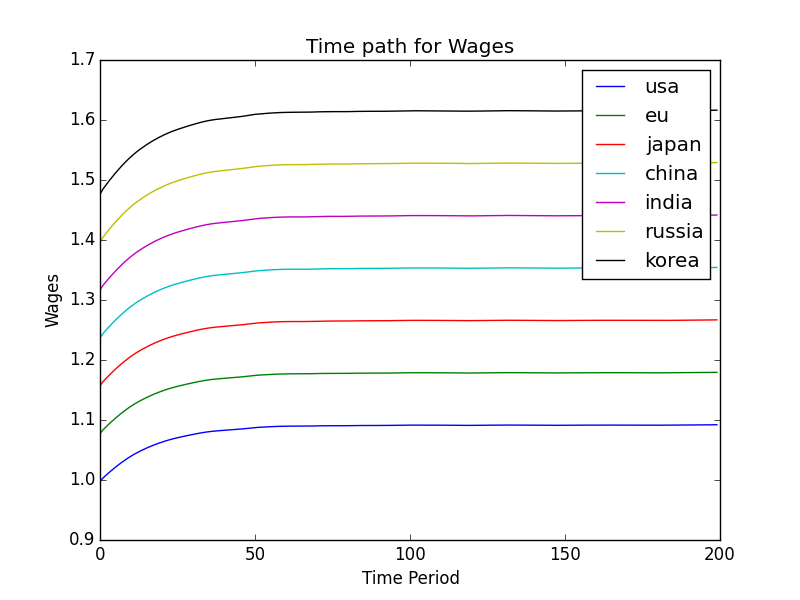
\includegraphics[scale=0.47]{wages.png}
\end{frame}

\begin{frame}
\frametitle{Global Interest Rate}
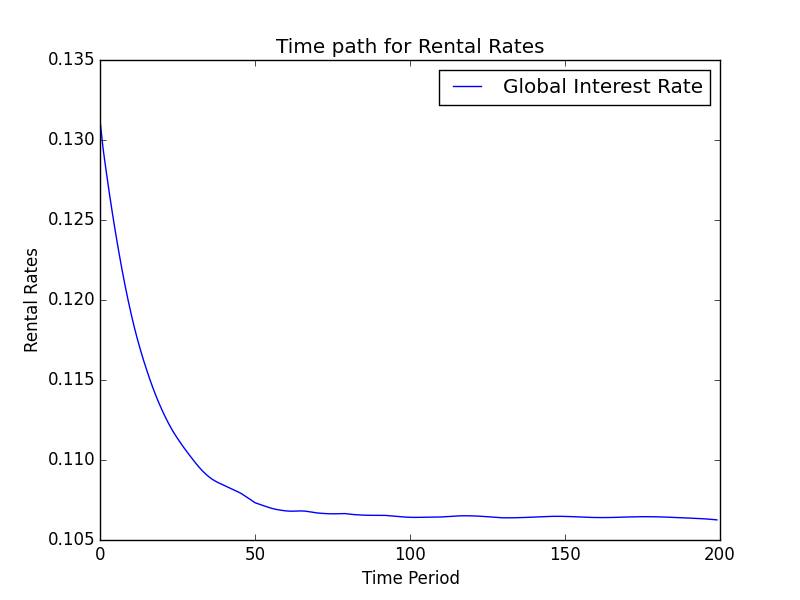
\includegraphics[scale=0.47]{rental_rate.png}
\end{frame}

\begin{frame}
\frametitle{Aggregate Output}
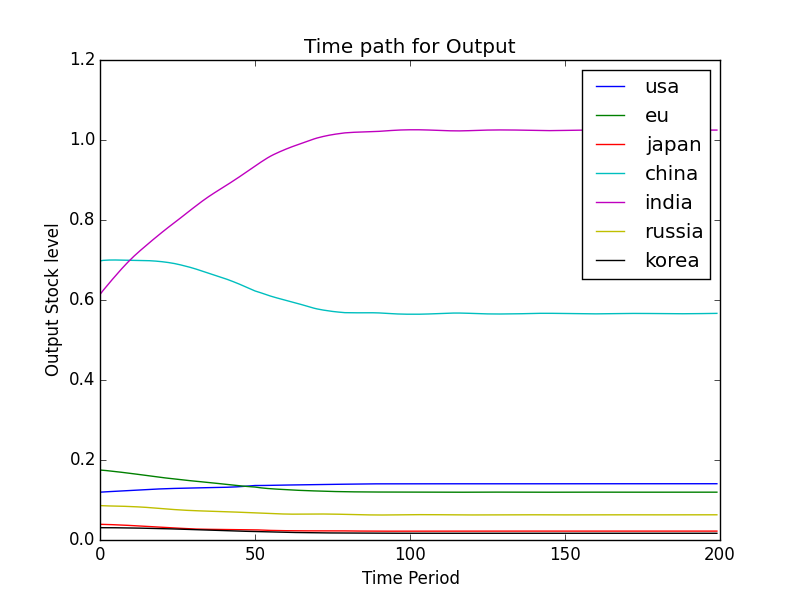
\includegraphics[scale=0.47]{output.png}
\end{frame}



\section{Future}


\frame{
\frametitle{Work To Be Done}
\begin{itemize}
\item This code is being built in stages, what we've shown is the first two stages.
\item Stage 3 (Current): Adding a Labor/Leisure Decision
\item Stage 4: Add children 
\begin{itemize}
\item Essentially, changing the utility function to reflect children's consumption, since people tend to value their children's consumption.
\end{itemize}
\item Stage 5: Adding Labor Classes

\item Stage 6: Adding Corporate Taxes
\vspace{3mm}


\end{itemize}
}

\end{document}
